\chapter{Maps for a mower}
\label{ch:maps}

The maps of the previous chapters are made for localisation: a few
thousand landmarks, each a point with a descriptor, enough to recognise
a place and compute a pose. They say nothing about where the mower may
drive or what it should cut. A coverage planner needs a different map:
every square decimetre of the garden classified as lawn to mow, ground
that can be crossed but not mowed (a path, a patio), or an obstacle;
and, as importantly, \emph{unknown} where the cameras have not looked.
This chapter builds that map from dense stereo depth and the keyframe
poses of the back-end, quantifies how the depth noise and the pose
errors limit it, and exports it in the format of the coverage planners
of the open-source Lawnmower project
(\url{https://github.com/CL-BZH/Lawnmower}).

\section{Two maps}

\begin{definition}{Mowing map}{mowmap}
A mowing map is a grid of square cells of side $c$ on the ground plane,
each with a class: \emph{mowable} (lawn that can be driven on),
\emph{obstacle} (cannot be entered), \emph{not lawn} (can be driven on
but not mowed), or \emph{unknown}. A \emph{planner grid} is a coarser
grid whose cells are the size of the blade's footprint, each either
mowable or blocked.
\end{definition}

The localisation map and the mowing map live side by side. The first is
sparse and precise, and it is what the pose graph optimises. The second
is dense and coarse, and nothing in it is optimised: it is \emph{fused}
from observations made at the keyframes. Each keyframe stores its own
classified points in its own camera frame. The grid is then a function
of the keyframe poses, and when a loop closure moves the keyframes, the
grid is rebuilt from the same observations at the new poses. Nothing
about the observations has to be redone, and a wrong loop that is later
rejected leaves no trace.

Richer dense maps exist --- point clouds, voxel grids, truncated signed
distance fields, 2.5D elevation maps --- and Further reading points to
them. A mower on a lawn needs to know where it can drive, which a 2D
grid with heights reduced to classes says directly.

\section{Dense stereo and its errors}

A dense stereo matcher (block matching, or semi-global matching) returns
a disparity for most pixels of the left image, not only at corners. The
simulation in \code{vslam/scene.py} ray-casts a model of the garden ---
the ground, the fence, house and shed as boxes, trees as cylinders, a
flower bed and a young tree in the lawn, a paved patio in one corner,
and a gravel border along the fence --- and returns the depth of every
fourth pixel with Gaussian disparity noise $\sigma_\delta=0.3$\,px and
5\,\% failed matches. On the lawn the surface it sees is the top of the
grass blades, up to 8\,cm above the soil.

\begin{proposition}{Covariance of a stereo point}{stereocov}
Let pixel $(u,v)$ have normalised coordinates $\vect{r}=(x,y,1)$ and
disparity $\delta$, so that $\vect{q}=Z\vect{r}$ with $Z=f_xb/\delta$.
If only the disparity is noisy, with standard deviation
$\sigma_\delta$, the first-order covariance of $\vect{q}$ is
\begin{equation}\label{eq:stereocov}
\Sigma_q=\sigma_Z^2\,\vect{r}\vect{r}\T,\qquad
\sigma_Z=\frac{Z^2}{f_xb}\,\sigma_\delta ,
\end{equation}
a rank-one matrix: the uncertainty lies along the ray.
\end{proposition}

\begin{proof}
$\vect{r}$ does not depend on $\delta$, so $\partial\vect{q}/\partial
\delta=\vect{r}\,\mathrm{d}Z/\mathrm{d}\delta=-\vect{r}\,Z^2/(f_xb)$
(\cref{prop:disparity}), and $\Sigma_q=(\partial\vect{q}/\partial\delta)
\,\sigma_\delta^2\,(\partial\vect{q}/\partial\delta)\T$.
\end{proof}

What matters for a map of the ground is how this error splits into a
height error and a horizontal error.

\begin{proposition}{Errors of a ground point}{grounderr}
Let the ground be the plane $\vect{n}\T\vect{q}=d$ in the camera frame,
with $\norm{\vect{n}}=1$ and the camera at height $h_c=-d>0$ above it.
A ground point at depth $Z$ has, to first order, a height error and a
horizontal error with standard deviations
\begin{equation}\label{eq:grounderr}
\sigma_h=\frac{h_c\,Z}{f_xb}\,\sigma_\delta,\qquad
\sigma_\parallel=\frac{Z^2}{f_xb}\,\sigma_\delta\,
\sqrt{\norm{\vect{r}}^2-h_c^2/Z^2}.
\end{equation}
\end{proposition}

\begin{proof}
The error is $\vect{r}\,\Delta Z$ with $\Delta Z$ of standard deviation
$\sigma_Z$. Its component along the normal is $(\vect{n}\T\vect{r})
\Delta Z$; since the point is on the ground, $\vect{n}\T\vect{r}=
\vect{n}\T\vect{q}/Z=d/Z$, so $\sigma_h=\sigma_Zh_c/Z$. The horizontal
component is $(I-\vect{n}\vect{n}\T)\vect{r}\,\Delta Z$, of norm
$\sqrt{\norm{\vect{r}}^2-(\vect{n}\T\vect{r})^2}\,|\Delta Z|$.
Substitute $\sigma_Z$ from \eqref{eq:stereocov}.
\end{proof}

\begin{inwords}
Seen from 80\,cm above, the ground is viewed at a grazing angle: the
ray to a point 4\,m away descends only $h_c/Z=0.2$ per metre. A depth
error slides the point along that ray, so it moves mostly
\emph{horizontally}. The height error grows like $Z$ and stays small
($1.7$\,cm at 4\,m with our rig); the horizontal error grows like $Z^2$
and is what limits the map.
\end{inwords}

Requiring $\sigma_\parallel\le c$, one grid cell, and taking
$\norm{\vect{r}}\approx1$ gives a maximum useful range
\begin{equation}\label{eq:maxrange}
Z_{\max}\approx\sqrt{\frac{c\,f_xb}{\sigma_\delta}} .
\end{equation}
For $c=10$\,cm, $f_xb=55$\,px\,m and $\sigma_\delta=0.3$\,px this is
$4.3$\,m. Points further away still carry information, but they smear
obstacles over several cells.

\section{The ground and the height of things}

To classify a point as ground or obstacle we need its height above the
ground. The world frame offers one ($z$), but only through the pose:
the VO's estimate of the gravity direction is off by about $1^\circ$
in our run (up to $1.4^\circ$), which moves a point 4\,m away by
7--10\,cm in height. On our flat simulated lawn this is still below
the obstacle threshold. On a real lawn, which slopes and bumps, the
plane $z=0$ is not the ground at all. Each keyframe therefore fits its
own ground plane to its own points.

\begin{proposition}{Total least squares plane}{tlsplane}
Let $\vect{p}_1,\dots,\vect{p}_m\in\R^3$ with centroid $\bar{\vect{p}}$
and scatter matrix $M=\sum_a(\vect{p}_a-\bar{\vect{p}})(\vect{p}_a-
\bar{\vect{p}})\T$. The minimiser of
\begin{equation}\label{eq:tls}
\sum_a\bigl(\vect{n}\T\vect{p}_a-d\bigr)^2\quad\text{subject to}\quad
\norm{\vect{n}}=1
\end{equation}
is $d=\vect{n}\T\bar{\vect{p}}$ with $\vect{n}$ a unit eigenvector of
$M$ for its smallest eigenvalue $\lambda_{\min}$, and the minimum is
$\lambda_{\min}$.
\end{proposition}

\begin{proof}
For fixed $\vect{n}$, the cost is a quadratic in $d$ whose derivative
$-2\sum_a(\vect{n}\T\vect{p}_a-d)$ vanishes at $d=\vect{n}\T
\bar{\vect{p}}$. Substituting, the cost becomes $\sum_a(\vect{n}\T
(\vect{p}_a-\bar{\vect{p}}))^2=\vect{n}\T M\vect{n}$. $M$ is symmetric
positive semidefinite; writing $\vect{n}$ in an orthonormal eigenbasis,
$\vect{n}\T M\vect{n}=\sum_k\lambda_kn_k^2\ge\lambda_{\min}\sum_kn_k^2=
\lambda_{\min}$, with equality for the eigenvector of
$\lambda_{\min}$.
\end{proof}

The distance $\vect{n}\T\vect{p}-d$ is measured perpendicular to the
plane, so all three coordinates are treated alike. This suits a
point cloud whose noise does not lie along one coordinate axis (by
\cref{prop:stereocov} it lies along the rays). Fitting the plane by
ordinary least squares, $Z$ as a function of $X$ and $Y$ say, would
treat two coordinates as exact.

\code{maps.ground\_plane} runs RANSAC on three-point planes, keeps only
planes within $10^\circ$ and 30\,cm of the plane predicted by the camera
mount, counts as inliers the points within 5\,cm (and 6\,m), and refits
on the inliers by \cref{prop:tlsplane}. The fitted plane runs over the
grass a few centimetres above the soil, which is what we want: heights
are measured from the surface the mower drives on. Its normal is not
more accurate than the VO's gravity direction: on our run it is off by
$0.7^\circ$ on average, because the grass tops are an uneven surface
and the inlier band is the same at 1\,m and at 6\,m (Exercise
\ref{ex:11thr}). Its advantage is that it is the ground under the
mower, whatever the slope. Each point within
the maximum range then gets a height $h=\vect{n}\T\vect{q}-d$ and a
kind:
\begin{itemize}[nosep]
\item ground if $|h|<15$\,cm (grass blades reach 8\,cm);
\item obstacle if $15\,\text{cm}\le h\le1.5$\,m;
\item ignored above 1.5\,m (branches, the upper wall of the house), as
  the mower passes under it, and below $-15$\,cm (outliers).
\end{itemize}
Ground points also carry the answer of a grass classifier, simulated as
correct 90\,\% of the time. In practice, colour and texture separate
grass from gravel and paving well in daylight.

\begin{figure}[ht]
\centering
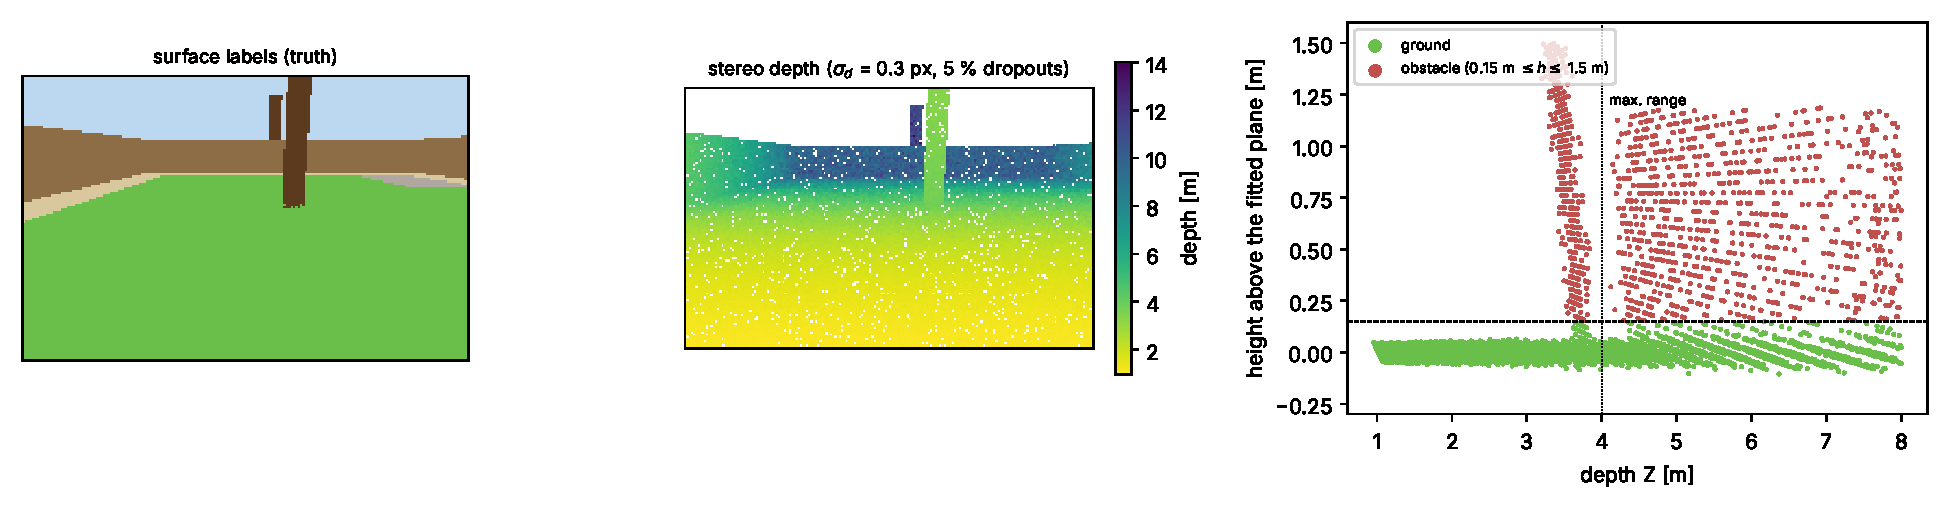
\includegraphics[width=\linewidth]{figures/ch11_frame.pdf}
\caption{One keyframe of the garden run. Left: the surfaces (lawn
green, gravel border beige, fence and trees brown). Middle: the stereo
depth. Right: heights of the points above the fitted ground plane; the
young tree at 3.5\,m and the fence beyond are obstacles. The scattered
red points past 4.5\,m are the fence, seen obliquely.}
\label{fig:frame11}
\end{figure}

\section{Occupancy grids}

\begin{definition}{Binary Bayes filter in log-odds}{logodds}
For a cell with binary state $m\in\{0,1\}$, the \emph{log-odds} of
$P(m=1\mid\z_{1:t})$ is $l_t=\log\frac{P(m=1\mid\z_{1:t})}
{1-P(m=1\mid\z_{1:t})}$. The prior is $l_0$, and an \emph{inverse
sensor model} $P(m=1\mid\z_t)$ gives the probability of the state
from one observation alone.
\end{definition}

\begin{proposition}{The log-odds update}{logoddsupdate}
If the cell does not change and the observations are conditionally
independent given $m$, then
\begin{equation}\label{eq:logodds}
l_t=l_{t-1}+\log\frac{P(m=1\mid\z_t)}{1-P(m=1\mid\z_t)}-l_0 .
\end{equation}
\end{proposition}

\begin{proof}
By Bayes' rule and conditional independence,
$P(m\mid\z_{1:t})=p(\z_t\mid m)P(m\mid\z_{1:t-1})/p(\z_t\mid
\z_{1:t-1})$, and by Bayes' rule again $p(\z_t\mid m)=P(m\mid\z_t)
p(\z_t)/P(m)$. Hence
\[
P(m\mid\z_{1:t})=\frac{P(m\mid\z_t)\,p(\z_t)\,P(m\mid\z_{1:t-1})}
{P(m)\,p(\z_t\mid\z_{1:t-1})}.
\]
Write this for $m=1$ and $m=0$ and divide: the factors that do not depend
on $m$ cancel, leaving
\[
\frac{P(m=1\mid\z_{1:t})}{P(m=0\mid\z_{1:t})}=
\frac{P(m=1\mid\z_t)}{P(m=0\mid\z_t)}\,
\frac{P(m=0)}{P(m=1)}\,
\frac{P(m=1\mid\z_{1:t-1})}{P(m=0\mid\z_{1:t-1})}.
\]
Taking logarithms gives \eqref{eq:logodds}.
\end{proof}

The update is a sum, so it is cheap, and a cell never seen keeps
$l=l_0$ (we take $l_0=0$). Two layers are kept per cell: occupancy
($m=1$: obstacle) and lawn ($m=1$: grass).

The independence assumption fails badly for the points that one
keyframe puts in one cell: they come from the same image, the same
pose, the same plane fit. Adding one update per point would make a cell
seen once by twenty points as certain as one seen by twenty keyframes.
\code{maps.LogOddsGrid} therefore gives each keyframe a single vote
per cell. The occupancy vote is ``obstacle'' ($P=0.8$) if at least
30\,\% of the cell's points are obstacles, and ``free'' ($P=0.3$)
otherwise. The lawn vote is ``grass'' or ``not grass'' ($P=0.75$) by
majority over the ground points. Votes from successive keyframes are
not independent either, but they are far less dependent than points
are.

\begin{proposition}{How fast votes settle a cell}{votes}
Let the votes on a cell be independent, each correct with probability
$1-\epsilon>\frac12$, and let a vote add $\pm a$ to the log-odds
($+a$ if it says $m=1$). If the true state is $m=0$, then after $n$
votes, with $l_0=0$,
\begin{equation}\label{eq:hoeffding}
P(l_n\ge0)\le\exp\bigl(-n(1-2\epsilon)^2/2\bigr).
\end{equation}
\end{proposition}

\begin{proof}
$l_n=\sum_{i=1}^nX_i$ with independent $X_i\in\{-a,+a\}$ of mean
$-a(1-2\epsilon)$. Hoeffding's inequality for variables in an interval
of length $2a$ gives $P\bigl(\sum X_i-\E\sum X_i\ge s\bigr)\le
\exp(-2s^2/(n(2a)^2))$. Take $s=na(1-2\epsilon)$.
\end{proof}

With the grass classifier ($\epsilon=0.1$), ten keyframes make a wrong
lawn label less likely than $\exp(-3.2)\approx4\,\%$, and twenty less
than $0.2\,\%$; the bound is loose, and the simulation does better. The
occupancy votes are asymmetric ($+1.39$ for a hit, $-0.85$ for a free
vote), so that obstacles are believed faster than free space, which is
the safe bias. The log-odds are clamped to $\pm6$ so that the map
remains able to change: a garden chair that is moved away needs
$(6+1.39)/0.85\approx9$ free votes before its cells drop below
$P=0.2$ and become mowable again.

A cell is then classified as \emph{obstacle} if $P(m_{\mathrm{occ}}=1)>
0.7$; \emph{mowable} if $P(m_{\mathrm{occ}}=1)<0.2$ and
$P(m_{\mathrm{lawn}}=1)>0.8$; \emph{not lawn} if $P(m_{\mathrm{occ}}=1)
<0.2$ and $P(m_{\mathrm{lawn}}=1)<0.2$; and \emph{unknown} otherwise.

\section{The pose matters}

\begin{figure}[ht]
\centering
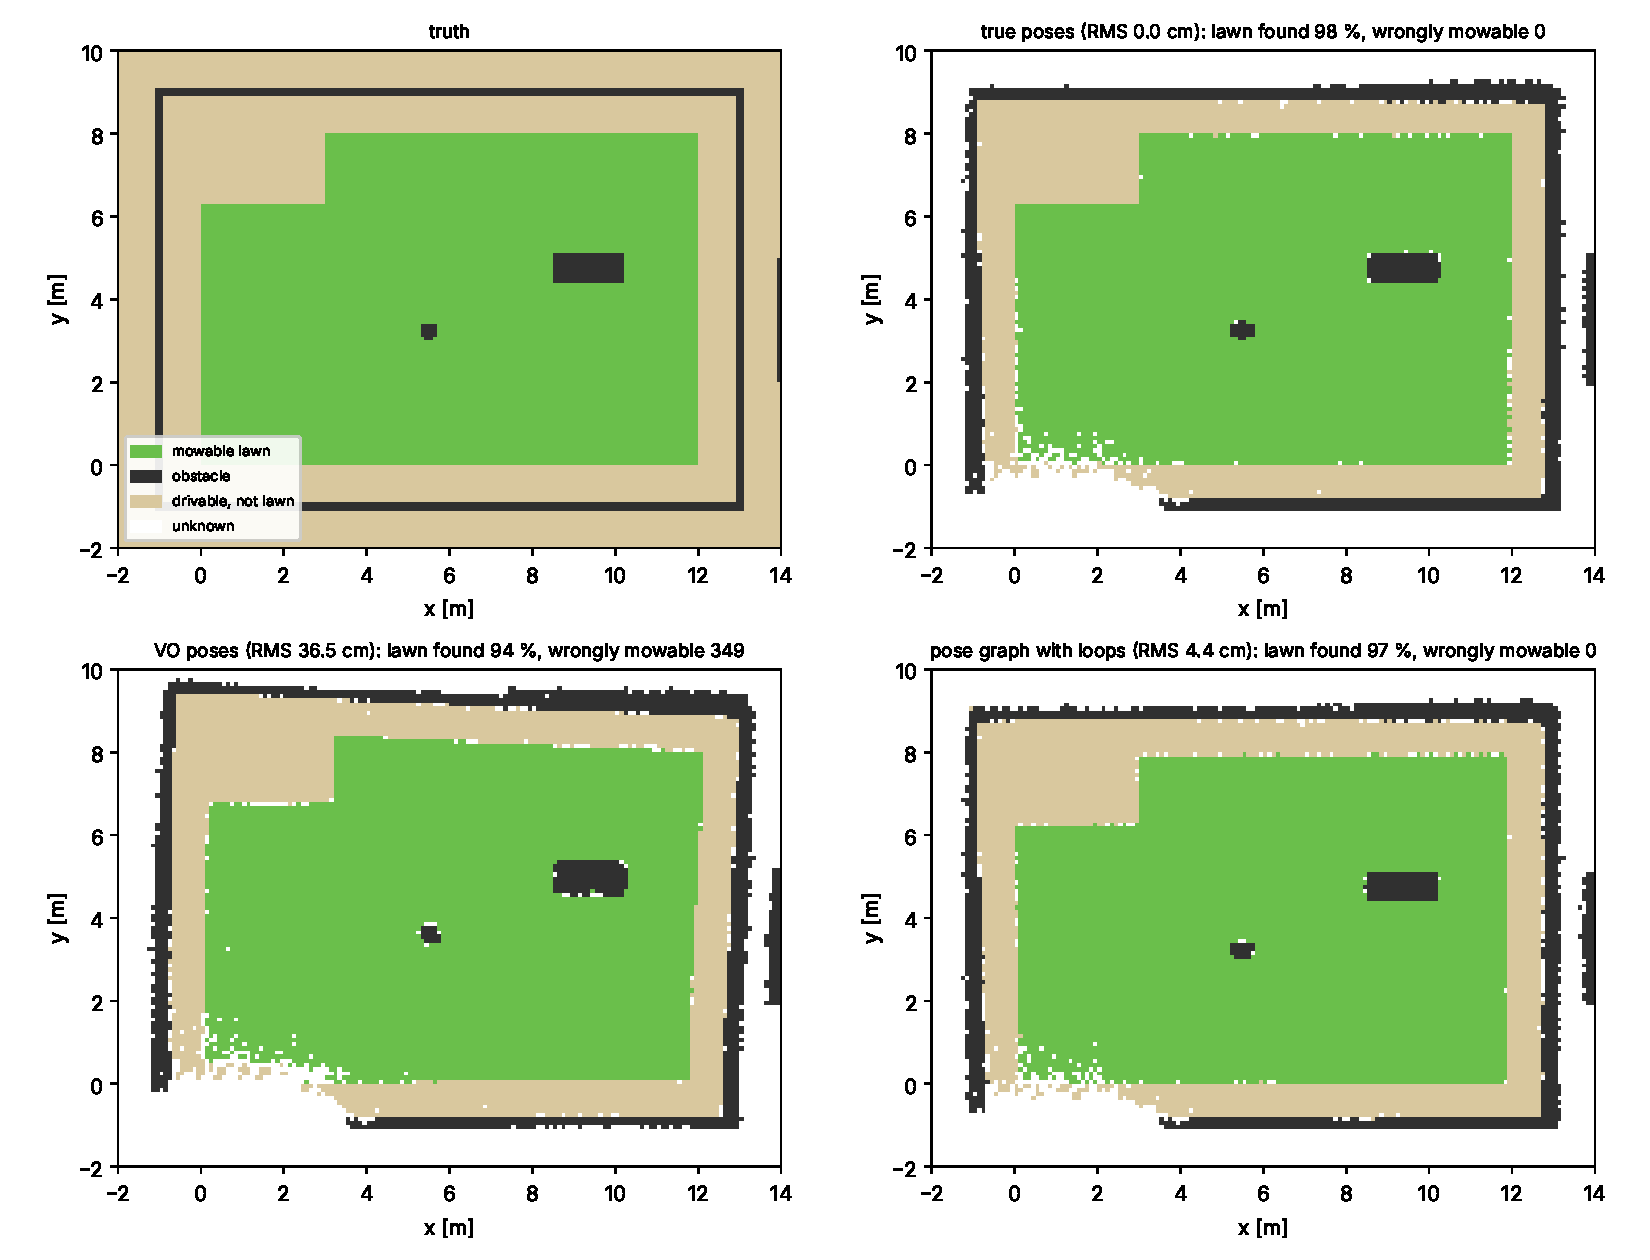
\includegraphics[width=\linewidth]{figures/ch11_maps.pdf}
\caption{Mowing maps (cells of 10\,cm) fused from the same keyframe
observations with three sets of poses: the truth, the VO of
Chapter~\ref{ch:vo}, and the pose graph corrected by the loops found in
Chapter~\ref{ch:loop}. ``Wrongly mowable'' counts cells inside the
fence that are obstacles or not lawn in truth but are classified
mowable.}
\label{fig:maps11}
\end{figure}

\Cref{fig:maps11} shows the map fused from the 153 keyframes of the
garden run. With the true poses, 98\,\% of the lawn is found mowable,
and no cell is wrongly mowable. With
the VO poses, whose error is 36.5\,cm RMS, the observations of
successive rows no longer agree. The patio and the gravel border bleed
into the lawn, 316 cells of not-lawn and 33 cells of obstacle become
mowable, and the flower bed and tree are smeared. With the poses of the
pose graph (4.4\,cm RMS), the map is nearly as good as with the truth:
96.5\,\% of the lawn found, and again no cell wrongly mowable.

A correct map is still not enough on its own: the planner must also
keep a margin around obstacles. The robot occupies a region
of the plane, not a point. Its \emph{configuration space} is obtained
by growing every obstacle by the robot's footprint (a Minkowski sum)
and by the uncertainty of its position. For a planner whose cell is the
blade footprint, this growth is already partly built in: a coarse cell
is blocked as soon as any of its fine cells is an obstacle.

\begin{figure}[ht]
\centering
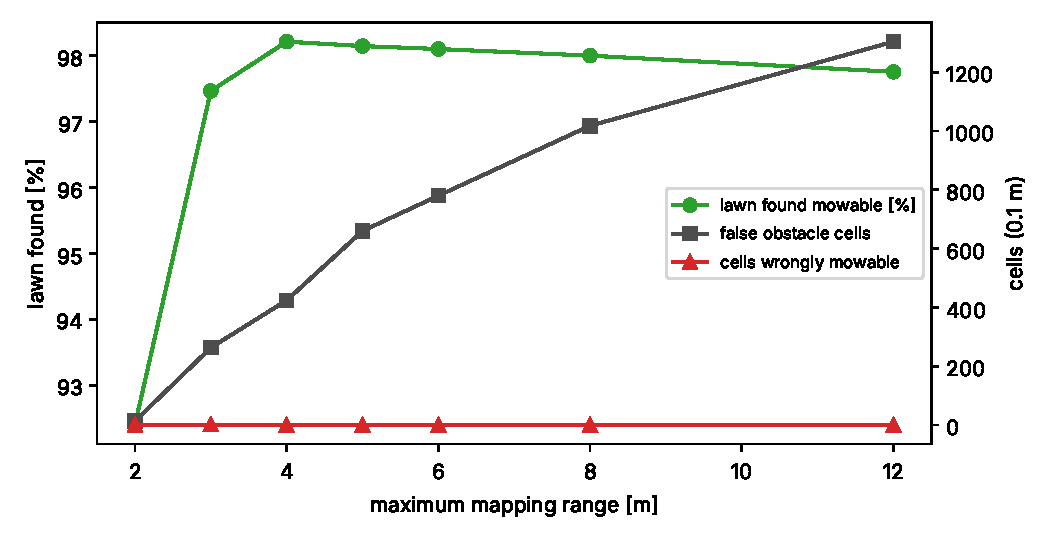
\includegraphics[width=0.72\linewidth]{figures/ch11_range.pdf}
\caption{Map quality with the true poses, as the maximum mapping range
varies. Beyond about 4\,m the lawn found no longer increases, while
obstacles keep growing, smeared by the horizontal depth error
\eqref{eq:grounderr}. At every range, at most one cell is wrongly
mowable.}
\label{fig:range11}
\end{figure}

\Cref{fig:range11} checks \eqref{eq:maxrange}. Up to 4\,m, a longer
range finds more lawn (92\,\% at 2\,m, 98\,\% at 4\,m). Beyond it, the
lawn found stays flat or decreases slightly, while the cells wrongly
marked as obstacles go from 424 at 4\,m to 1304 at 12\,m: obstacles
swell, as $\sigma_\parallel$ grows like $Z^2$. The mapping code uses
4\,m, the value the proposition predicts.

\section{From the map to the planner}

The Lawnmower planners take a text grid in which one character is one
cell of the size the blade cuts: \code{L} lawn, \code{S} the start,
\code{+} blocked. \code{maps.coarsen} groups $10\times10$ fine cells
into one cell of 1\,m, close to the cutting width of a ride-on deck. A
coarse cell is mowable only if at least 90\,\% of its fine cells are
mowable and none is an obstacle; unknown cells count against it.
\code{maps.to\_lawn\_text} writes the result, north at the top.

\begin{figure}[ht]
\centering
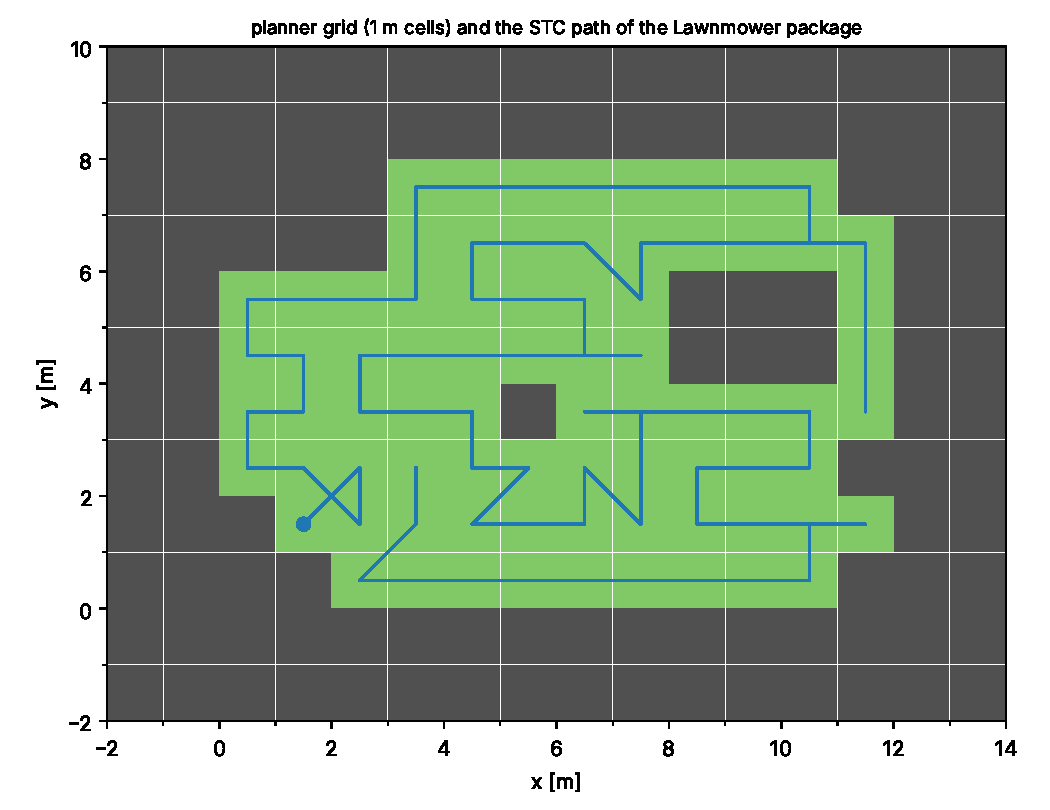
\includegraphics[width=0.62\linewidth]{figures/ch11_plan.pdf}
\caption{The planner grid (1\,m cells) from the map of the pose graph,
and the path of the spanning-tree coverage planner of the Lawnmower
package, started at the dot near $(1.5,1.5)$.}
\label{fig:plan11}
\end{figure}

From the map of the pose graph, 77 cells are mowable, against 83 in
truth, and none of them wrongly. The cells lost are those along the
edges, where a 1\,m cell overlaps the border by a few centimetres.
The spanning-tree coverage planner (STC) of the Lawnmower package covers
all 77 in 83 moves, with 7 revisits (\cref{fig:plan11}). A lawn edge
that the conservative planner grid leaves uncut is the job of a second,
finer pass along the boundary, the way a person mows the edge after the
rows.

\begin{mower}
Three consequences for the mower. First, the obstacle threshold of
15\,cm should come from the machine, not from this chapter: the deck's
ground clearance and the height of anything the blade must not touch
(sprinkler heads, roots, garden lights) set it. Second, the map is made
for planning, not for safety: people, children, pets and a forgotten
hose are not in yesterday's map. The live depth image should be checked
for obstacles in the mower's path at every frame, independently of the
map, with a bumper and an emergency stop below that. Third, the map is
anchored to keyframes, so a loop closure or the RTK-GNSS correction of
Chapter~14 improves the map for free, by re-fusion.
\end{mower}

\begin{practice}[\code{vslam/scene.py}, \code{vslam/maps.py},
  \code{examples/ch11\_maps.py}, \code{notebooks/ch11\_maps.ipynb}]
\begin{center}
\begin{tabular}{@{}ll@{}}
\toprule
Code & Formula\\
\midrule
\code{scene.Garden.raycast}, \code{render\_stereo} & dense stereo
  simulation\\
\code{maps.point\_covariance} & \cref{prop:stereocov}\\
\code{maps.fit\_plane\_tls}, \code{ground\_plane} & \cref{prop:tlsplane}
  in RANSAC\\
\code{maps.classify\_points} & heights, \eqref{eq:maxrange}\\
\code{maps.LogOddsGrid} & \cref{prop:logoddsupdate}, one vote per
  keyframe\\
\code{maps.fuse} & re-fusion with new poses\\
\code{maps.coarsen}, \code{to\_lawn\_text} & planner grid, Lawnmower
  format\\
\bottomrule
\end{tabular}
\end{center}
The tests check the TLS plane and its orientation, the stereo point
covariance against Monte Carlo (and its rank), ray casting against the
ground, the fence and the sky, the ground plane of a rendered keyframe
against the true one, the log-odds update against Bayes' rule computed
by hand, that coarsening is conservative, the orientation of the text
export, and (if the Lawnmower package is installed) that the export
loads and is fully covered by a planner. The notebook adds the error
propagation of \cref{prop:grounderr} against Monte Carlo and the vote
bound of \cref{prop:votes}.
\end{practice}

\section*{Further reading and C++ pointers}
\addcontentsline{toc}{section}{Further reading and C++ pointers}

Occupancy grids: H.~Moravec and A.~Elfes (ICRA 1985), A.~Elfes (IEEE
Computer 1989), and chapter~9 of \emph{Probabilistic Robotics} by
S.~Thrun, W.~Burgard and D.~Fox. Semi-global matching: H.~Hirschm\"uller
(IEEE TPAMI 2008). Volumetric maps: OctoMap (A.~Hornung et~al.,
Autonomous Robots 2013); truncated signed distance fields: KinectFusion
(R.~A.~Newcombe et~al., ISMAR 2011) and Voxblox (H.~Oleynikova et~al.,
IROS 2017). Elevation maps for rough terrain: P.~Fankhauser et~al.
(\code{grid\_map} and \code{elevation\_mapping}). Coverage path
planning: the survey of E.~Galceran and M.~Carreras (Robotics and
Autonomous Systems 2013) and STC (Y.~Gabriely and E.~Rimon, Annals of
Mathematics and Artificial Intelligence 2001). In C++:
\code{cv::StereoSGBM} for dense disparity, PCL for plane RANSAC,
OctoMap, \code{grid\_map}, and Nav2's costmaps in ROS~2.

\FloatBarrier
\section*{Exercises}
\addcontentsline{toc}{section}{Exercises}

\begin{enumerate}[label=\textbf{11.\arabic*},ref=11.\arabic*]
\item\label{ex:11range} Evaluate \eqref{eq:maxrange} for
  $\sigma_\delta=0.5$\,px, and for a rig with a 30\,cm baseline. What
  else changes with the longer baseline?
\item\label{ex:11thr} The RANSAC inlier threshold of the ground plane is
  a constant 5\,cm. Using \cref{prop:grounderr}, propose a threshold that
  depends on $Z$, and compute it at 1\,m and 6\,m.
\item\label{ex:11chair} With the clamp at $\pm6$, a hit adding $1.39$
  and a free vote $-0.85$, how many free votes turn a saturated
  obstacle cell mowable ($P<0.2$)? How many hits make a saturated free
  cell an obstacle ($P>0.7$)? Comment on the asymmetry.
\item\label{ex:11pervote} Suppose each keyframe put one update per
  \emph{point} in a cell, with 20 points per cell and per keyframe, and
  the points of one keyframe always agree. What would \eqref{eq:logodds}
  then claim after one keyframe, and why is it wrong?
\end{enumerate}

\subsection*{Solutions}

\textbf{11.1.} With $\sigma_\delta=0.5$\,px: $Z_{\max}=\sqrt{0.1\cdot
55/0.5}=3.3$\,m. With $b=0.3$\,m, $f_xb=138$\,px\,m and, at
$\sigma_\delta=0.3$\,px, $Z_{\max}=\sqrt{0.1\cdot138/0.3}=6.8$\,m: the
range grows like $\sqrt b$. The price is near-field coverage: the two
images overlap only beyond a larger distance, and very close objects
(the most dangerous ones for a mower) are seen by one camera only; the
disparities of near points also become large, and the matcher's
search range must grow.

\textbf{11.2.} The plane's inliers should be the points within a few
standard deviations of the grass surface: a threshold $\tau(Z)=
\tau_0+k\sigma_h(Z)$ with $\tau_0$ for the grass (a few centimetres)
and $\sigma_h=h_cZ\sigma_\delta/(f_xb)$. With $h_c=0.8$\,m,
$\sigma_\delta=0.3$\,px, $f_xb=55$\,px\,m and $k=3$: $3\sigma_h=1.3$\,cm
at 1\,m and $7.8$\,cm at 6\,m. A constant 5\,cm is generous near the
mower and too tight far away, which is one reason the fit uses only
points within 6\,m.

\textbf{11.3.} From $+6$, free votes reach $\mathrm{logit}(0.2)=-1.39$
after $n>(6+1.39)/0.85=8.7$, i.e.\ 9 votes. From $-6$, hits reach
$\mathrm{logit}(0.7)=0.85$ after $n>(6+0.85)/1.39=4.9$, i.e.\ 5 votes.
An obstacle appears about twice as fast as it disappears: a false
obstacle costs some uncut grass, a missed one can cost a blade or worse.

\textbf{11.4.} With the per-keyframe inverse model $P=0.8$, each point
would add $1.39$: one keyframe would bring the cell to $l=27.7$, i.e.\
$P(\text{obstacle})=1-10^{-12}$, from a single image and a single plane
fit. The twenty points are not independent observations: they share
the pose, the plane and any systematic error of that keyframe (a wrong
plane, a shadow misread by the grass classifier). The posterior should
be close to that of one observation, which one vote per keyframe gives.
